\documentclass[
 aip,
 jmp,
 amsmath,amssymb,
 reprint,
]{revtex4-1}
\usepackage{graphicx}
\usepackage{grffile}
\usepackage{dcolumn}
\usepackage{bm}
\usepackage{multirow}
\usepackage{color}
\begin{document}
\preprint{AIP/123-QED}
\title[A quantitative approach to humanities evolution and two case studies]{A quantitative approach to humanities evolution and two case studies}
\author{Vilson Vieira}
 \homepage{http://automata.cc}
 \email{vilson@void.cc}
\author{Renato Fabbri}
 \homepage{http://www.estudiolivre.org/el-user.php?view\_user=gk}
 \email{renato.fabbri@gmail.com}
\author{Gonzalo Travieso}
  \email{gonzalo@ifsc.usp.br}
  \affiliation{ 
Instituto de F\'isica de S\~ao Carlos, Universidade de S\~ao Paulo (IFSC/USP)
}
\author{Luciano da Fontoura Costa}
  \homepage{http://cyvision.ifsc.usp.br/~luciano/}
  \email{ldfcosta@gmail.com}
  \affiliation{ 
Instituto de F\'isica de S\~ao Carlos, Universidade de S\~ao Paulo (IFSC/USP)
}
\date{\today}
\begin{abstract}
We propose a
methodology
to study humanities development by
applying multivariate statistics on two case studies: composers and philosophers.
Seven representative composers and philosophers were considered in terms of
eight main musical and philosophical features. 
Grades
were assigned to each characteristic and their correlations were
analyzed. 
A bootstrap method was
applied to avoid statistical biasing caused by the small sample data set, simulating hundreds of artificial composers and philosophers
influenced by the seven representatives chosen.
Afterwards we quantify non-numeric relations like dialectics, opposition
and innovation on both fields.
Composers and philosophers differences on style and technique were represented
as geometrical distances in the feature space, making it possible to
quantify, for example, how much Bach and Stockhausen differ from other composers, how
much Beethoven influenced Brahms or how much was Spinoza in opposition of their contemporaries.
In addition, we compared the results on both fields. Opposition, strong on
philosophy, was not remarkable on music. Supporting an observation already considered by music
theorists, strong influences were identified between
composers by the quantification of dialectics, implying inheritance and suggesting a stronger
master-disciple evolution when compared to the philosophy analysis.
\end{abstract}
\pacs{89.75.Fb,05.65.+b} % PACS, the Physics and Astronomy
\keywords{music, musicology, pattern recognition, statistics}
\maketitle

\section{\label{sec:level1}Introduction}

In the history of music, composers developed their own styles along a
continuous search for coherence or unity. In the words of Anton
Webern~\cite{Webern}, ``[...] ever since music has been written most great artists
have striven to make this unity ever clearer. Everything that has
happened aims at this [...]''. Along this process we can identify
a constant heritage of style from one composer to another as
a gradual development from its
predecessor, contrasting with the necessity for innovation. Quoting
Lovelock: 
``[...] by experiment that progress is possible; it is the man
with the forward-looking type of mind [...] who forces man out of the
rut of `what was good enough for my father is good enough for me'.''~\cite{Lovelock}.
Thus, development in music follows a dichotomy: while composers aims on
innovation, creating their own styles, their technique is based on the
works of their predecessors, in a master-apprentice tradition.

Other fields like philosophy demonstrate
a well-defined trend when considering innovation: unlike music, the
quest for difference seems to drive philosophical
changes as expressed by Gilles Deleuze~\cite{Deleuze}. In other approaches such as Ferdinand de
Saussurre's principle~\cite{Saussure}, concepts (words) tend
to be different in the sense of meaning distinct things.  The paradigm
of difference is particularly promising because it is immediately
related to the own dynamics of philosophical evolution along time.  In
other words, what are the forces that drive philosophical changes and
innovation?  Could dialectics account for some of the main
philosophical moves? Are these concepts present on other fields like music?

In order to try and answer these questions, on both humanities fields in a more objective way, we resorted to a quantitative approach which turned out to provide a number of remarkable spin-offs and insights. More specifically, we
started by identifying prominent music composers and philosophers along the history, a set of main musical and philosophical issues, and then
assign grades to each of these issues for the chosen composers and philosophers. It is important to argue that the grades assignment was not arbitrary. The scores was not assigned on a random way but based on a historical research about techniques and styles used by both composers and philosophers. The grades reveals a \emph{tendency index} about particular characteristics of each composer or philosopher. For example, to say that Bach is more contrapuntist than the other remarkable composers is the same to give a bigger grade -- around 8.0 or 9.0 -- to the Barroque master and smaller grades to the others.

It should be stressed that we chose a reduced set of philosophers for the
sake of simplicity and clarity. Considering this
small number of philosophers and composers we developed a bootstrap method~\cite{Varian} to avoid a statistical biasing caused by the small number of samples. In this way we generated a larger data set of 1000 new \emph{artificial composers and philosophers} directly influenced by the originals samples, representing the contemporaries of the representatives chosen.

Those scores assigned to each composer - and philosopher - characteristics define a state vector in its feature space. This quantification of composers and philosophers characteristics paved the way to the application of sound concepts and methods from multivariate statistics~\cite{Papoulis, Wichern,
Therrien} and pattern recognition~\cite{Duda, Costa}. Correlations between these characteristic vectors were identified and principal component
analysis (PCA)~\cite{Costa} is applied to
represent the musical - and philosophical - history as a planar space where we can follow the historical development as vectorial movements. On this planar space, concepts like dialects, innovation and opposition, originally non-quantitative, can be modeled as mathematical relations between the individual states. By proposing indices to quantify the
degree of opposition, skewness and dialectics along the dynamics of
musical and philosophical individual evolutions, we observed surprising results.

It is important to note that application of statistical analysis to
music is not recent. On musicology, statistical methods have been used
to identify many musical characteristics.
Simonton~\cite{Simonton1991829, Simonton1977791} used time-series analysis to measure the creative productivity
of composers based on their music and popularity. Kozbelt~\cite{Kozbelt01012009, Kozbelt01012007} also
analyzed the productivity, but based on the measure of performance
time of the compositions and investigated the relation between
productivity and versatility. More recent works~\cite{Kranenburg2004, Kranenburg2007} use machine-learning
algorithms to recognize musical styles of selected compositions. 
Differently from these works, we are not interested in applying
statistical analysis to music but on characterizing composers by the identification of scores based on their recognized styles. On the other hand, automatic information retrieval, common on music, is not common on philosophy. The method proposed here is a way to analyze both fields indenpendently of the nature of their final products -- e.g.\ music pieces and textual documents -- but based on a well-formed opinion of reviewers on these fields.

This work starts by presenting the methodology adopted and then
presents the seven composers and philosphers followed by the definition of the eight musical and philosophical characteristics chosen. The proposed method was applied on these data sets, allowing us to compare both fields and discuss the results.

\section{Mathematical Description}

The choice of composers and philosophers is inherently important for the
time-evolution analysis, as each musical and philosophical move and its
characteristics (i.e.\ opposition and skewness) are defined by each
pair of subsequent composer or philosophers along time.  We decided to choose the
composers and philosophers taking into account their historical importance and
visibility. 

%% A sequence $S$ of $P$ philosophers along a given period
%% of time would incorporate the $P$ most prominent and visible
%% philosophers in that interval.  The use of such a criterion to build
%% the time-sequence for the philosophers implies in not necessarily
%% uniform time-intervals between each pair of subsequent entries. The same to the $C$ composers.

A sequence $S$ of $C$ music composers and $P$ philosophers was chosen based on their
relevance at each period of the classical music history and western philosophy history, respectivelly. The set of $C$ measurements
define a $C$-dimensional space henceforth referred as the \emph{musical space}. By the same way we defined a $P$-dimensional \emph{philosophical space} based on $P$ measurements.  

The characteristic vector $\vec{v}_i$ of each composer or philosopher $i$ defines a respective \emph{composer state} in the musical space or \emph{philosopher state} in the philosophical space. For the set of
$C$ composers, we defined the same relations adapted for the set of $P$ philosophers, sumarized in Table \ref{tab:tableRelations}. 

\begin{table}
\caption{\label{tab:tableRelations}Description of mathematical relations defined for each composer or philosopher $i$, $j$ and $k$ given a set of $C$ composers or $P$ philosophers as a time-sequence $S$.}
\begin{ruledtabular}
\begin{tabular}{ll}
\\ Average state & $\vec{a}_i = \frac{1}{i}\sum_{k=1}^i\vec{v}_k.$ \\ \\
Opposite state & $\vec{r}_i = \vec{v}_i + 2(\vec{a}_i - \vec{v}_i)$ \\ \\
Opposition vector & $\vec{D}_i=\vec{r}_i - \vec{v}_i$ \\ \\
Musical or \\ philosophical move & $\vec{M}_{i,j} = \vec{v}_j - \vec{v}_i$ \\ \\
Opposition index & $W_{i,j} = \frac{\left< \vec{M}_{i,j}, \vec{D}_i\right>}{||\vec{D}_i||^2}$ \\ \\
Skewness index & $s_{i,j} = \sqrt{\frac{|\vec{v}_i-\vec{v}_j|^2|\vec{a}_i-\vec{v}_i|^2 - [(\vec{v}_i-\vec{v}_j) . (\vec{a}_i-\vec{v}_i)]^2}{|\vec{a}_i-\vec{v}_i|^2}}$ \\ \\
Counter-dialectics \\ index & $d_{i \rightarrow k} = \frac{|\left< \vec{v}_j-\vec{v}_i,\vec{v}_k \right> + \frac{1}{2}\left<\vec{v}_i-\vec{v}_j, \vec{v}_i+\vec{v}_j\right>|}{|\vec{v}_j-\vec{v}_i|}$
\end{tabular}
\end{ruledtabular}
\end{table}

It is important to note some details about these relations. Here we are focusing on composers, but the same is valid for philosophers or characteristic vectors defined from other fields. Given a set of $C$ composers as a time-sequence $S$, the \emph{average state} at time $i$ is defined. The \emph{opposite state} is defined as the ``counterpoint'' of a musical state $\vec{v}_i$, considering its average state: everything running along the opposite direction of $\vec{v}_i$ are understood as opposition. In other words, any displacement from $\vec{v}_i$ along the direction $\vec{r}_i$ is a \emph{contrary move}, and any displacement from $\vec{v}_i$ along the direction $-\vec{r}_i$ is an \emph{emphasis move}. Given a musical state $\vec{v}_i$ and its opposite state $\vec{r}_i$, we can define the \emph{opposition vector} $\vec{D}_i$. These details are better understood analyzing Figure \ref{fig.1}.

\begin{figure}
        \begin{center}
                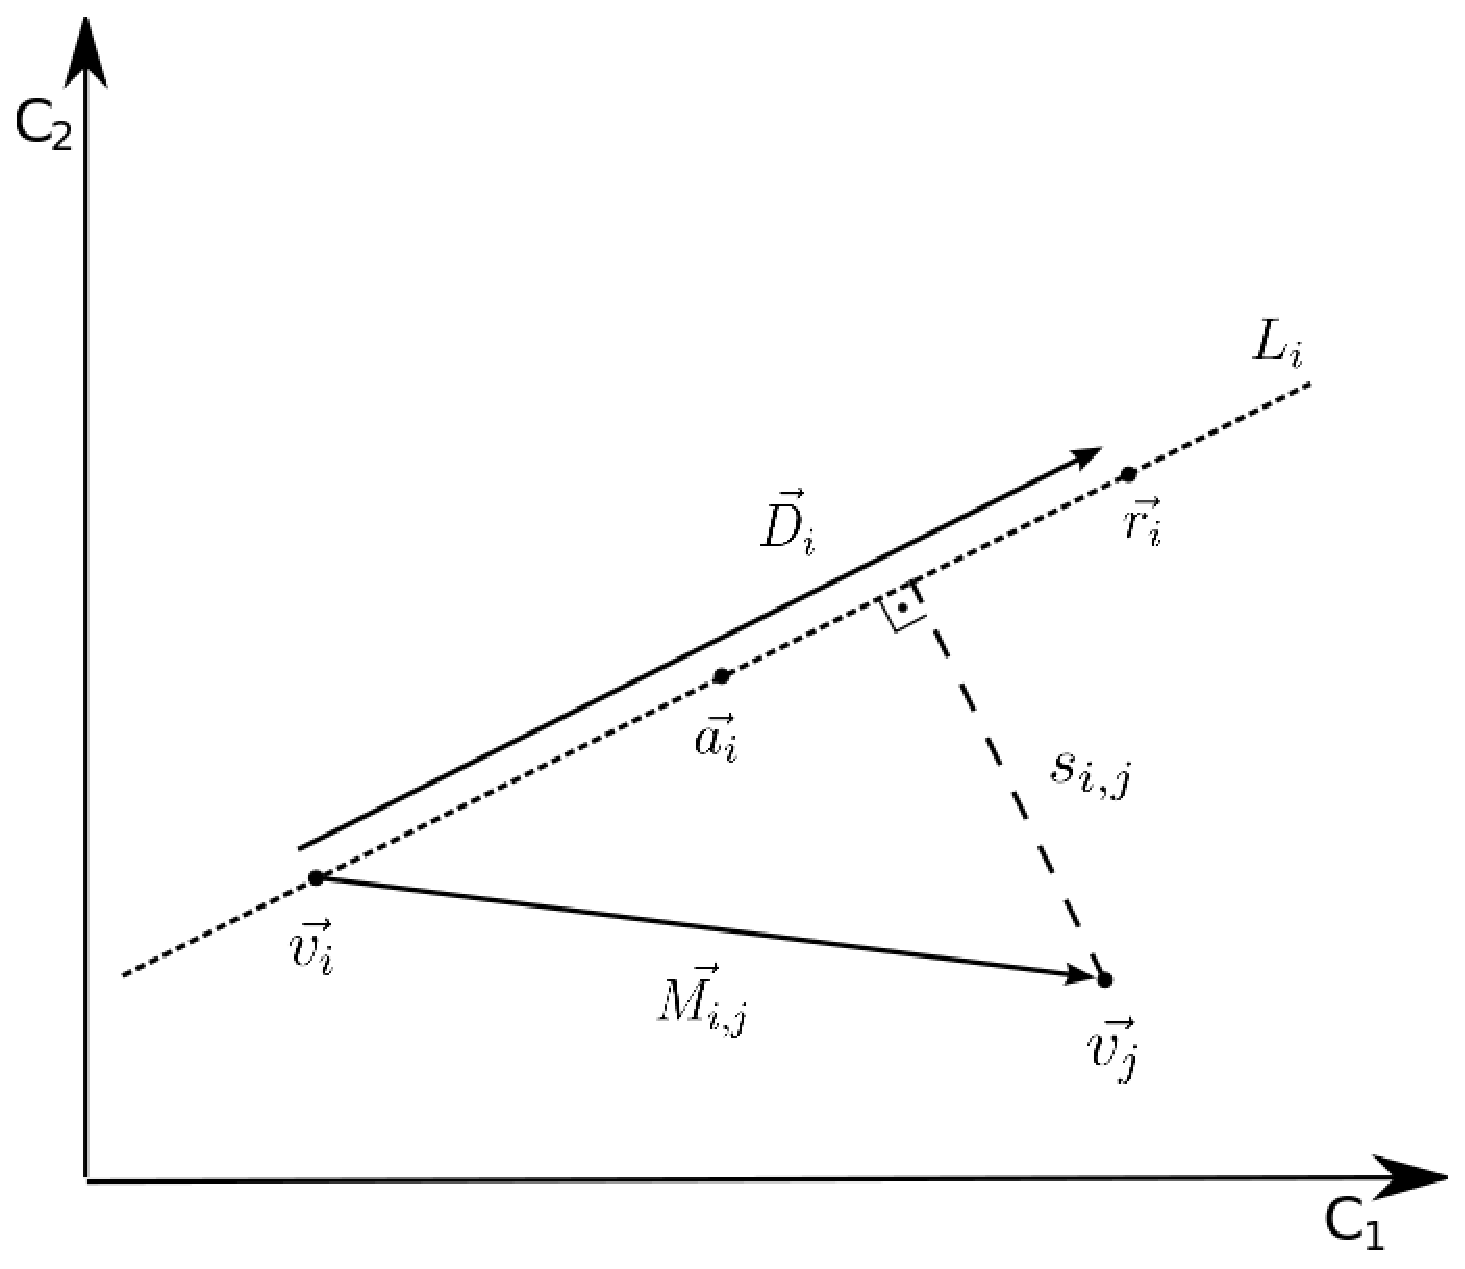
\includegraphics[width=0.35\textwidth]{phil-space-desc_}
        \end{center}
        \caption{\it Graphical representation of the measures derived from a \emph{musical move}.}
        \label{fig.1}
\end{figure}

Considering the time-sequence $S$ we defined relations between pairs of composers. The \emph{musical move} implied by two successive composers at time $i$ and $j$ corresponds to the $\vec{M}_{i,j}$ vector extending from $\vec{v}_i$ to $\vec{v}_j$. Given the musical move we can quantify the intensity of opposition by the projection of $\vec{M}_{i,j}$ along the opposition vector $\vec{D}_i$, normalized, yelding the \emph{opposition index}. Considering the same musical move, the \emph{skewness index} is the distance between $\vec{v}_j$ and the line $L_i$ defined by the vector $\vec{D}_i$, and therefore quantifies how much the new
musical state departs from the respective opposition move.

A relationship between a triple of successive composers can also be defined. Considering $i$, $j$ and $k$ being respectively understood as the \emph{thesis}, \emph{antithesis} and \emph{synthesis}, we defined the \emph{counter-dialectics index} by the distance between the musical state $\vec{v}_k$ and the middle line $ML_{i,j}$ defined by the thesis and antithesis, as shown in Figure \ref{fig.2}. In higher dimensional philosophical spaces,
the middle-hyperplane defined by the points which are at equal
distances to both $\vec{v}_i$ and $\vec{v}_j$ should be used instead
of the middle line $ML_{i,j}$. The proposed equation for counter-dialectics scales to hyperplanes.

The counter-dialectics index is suggested and used instead of dialectics index to maintain compatibility with the use of a distance from point to line as adopted for the definition of skewness.

\begin{figure}
        \begin{center}
                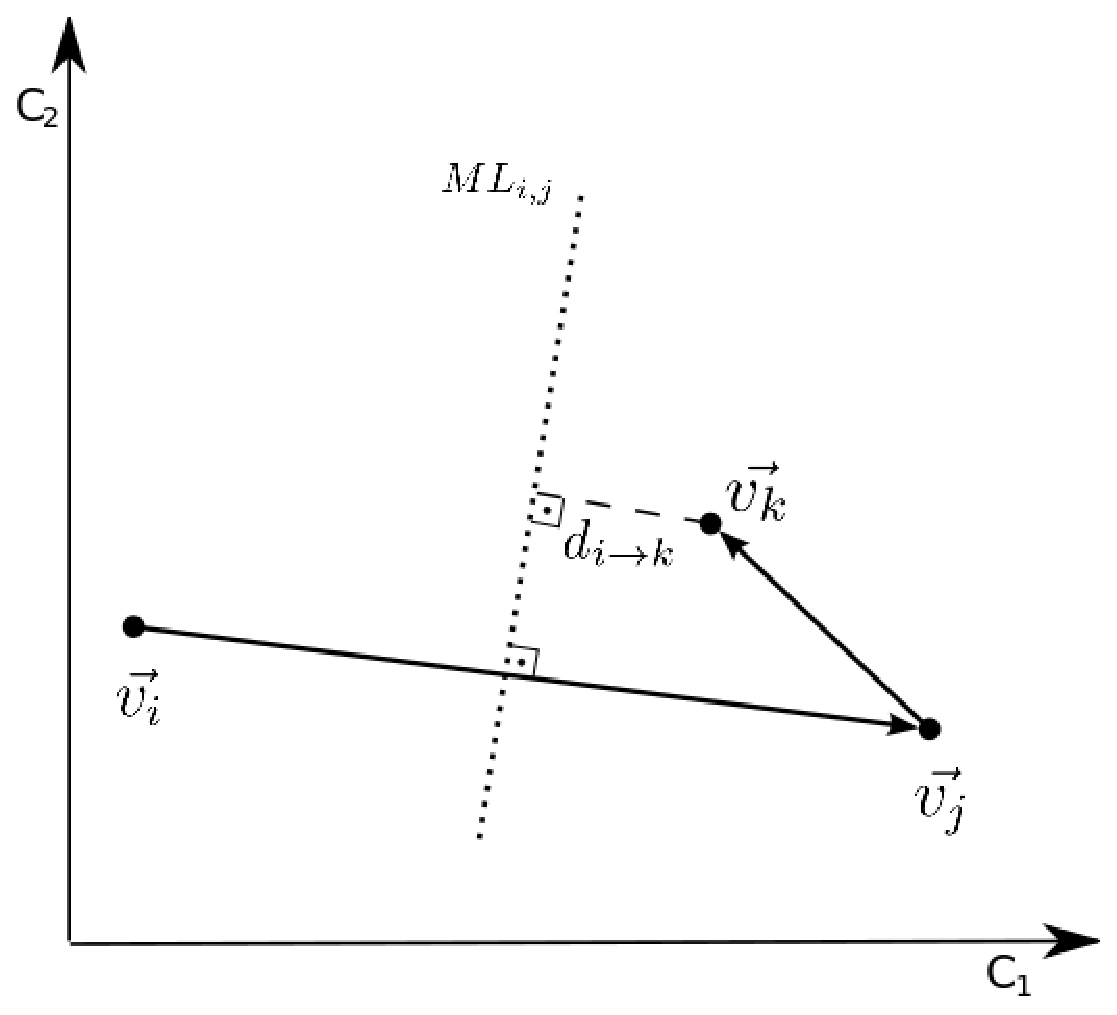
\includegraphics[width=0.35\textwidth]{dialetica_.eps}
        \end{center}
        \caption{\it Graphical representation of the quantification of dialectics.}
        \label{fig.2}
\end{figure}

\section{Characteristics}

To create the musical and philosophical space we derived eight variables corresponding to
distinct characteristics commonly found in music compositions and philosophers works. 

\subsection{Musical Characteristics}

The
characteristics are related with the basic elements of music --- melody,
harmony, rhythm, timbre, form and tessitura~\cite{BennettHistory} --- and
non-musical issues like historical events that have influenced the
compositions, for example, the
presence of Church. All the eight
characteristics are listed below:

{\bf \em{ Sacred - Secular}} ($S$-$S_c$): the sacred or religious music is
composed through religious influence or used for its purposes. \textit{Masses},
\textit{motets} and hymns, dedicated to the Christian liturgy, are well known examples~\cite{Lovelock}. Secular
music has no or little relation with religion and includes
popular songs like Italian madrigals and German \textit{lieds}~\cite{BennettHistory}. 

{\bf \em{ Short duration - Long duration}} ($D_s$-$D_l$): compositions are
quantified having short duration when they do not have more than few minutes
of execution. Long duration compositions have at least 20 minutes of execution or
more. The same consideration was adopted by Kozbelt~\cite{Kozbelt01012009,
  Kozbelt01012007} in his analysis of time execution.

{\bf \em{ Harmony - Counterpoint}} ($H$-$C$): harmony regards the
vertical combination of notes, while counterpoint focuses on
horizontal combinations~\cite{BennettHistory}.

{\bf \em{ Vocal - Instrumental}} ($V$-$I$): compositions using just vocals
(e.g.\ \emph{cantata}) or exclusively instruments
(e.g.\ \emph{sonata}). It is interesting to note the use of
vocals over instruments on Sacred compositions~\cite{Lovelock}.

{\bf \em{ Non-discursive - Discursive}} ($D_n$-$D$): compositions
based or not
on verbal discourse, like programmatic music or Baroque rhetoric, where the composer wants
to ``tell a history'' invoking images to the listeners
mind~\cite{BennettHistory}. Its contrary part is known as
\textit{absolute music} where the music is written to be appreciated simply
by what it is.

{\bf \em{ Motivic Stability - Motivic Variety}} ($M_s$-$M_v$): motivic pieces presents equilibrium
between repetition, reuse and variation of melodic motives. Bach is noticeable by his
\textit{development by variation} of motives, contrasting with the
constantly inventive use of new materials by Mozart~\cite{Webern}.

{\bf \em{ Rhythmic Simplicity - Rhythmic Complexity}} ($R_s$-$R_c$): presence or not of polyrhythms, the
use of independent rhythms at the same time --- also known as
\textit{rhythmic counterpoint}\cite{BennettHistory} --- a characteristic
constantly found in Romanticism and the works of 20th-century composers like Stravinsky.

{\bf \em{ Harmonic Stability - Harmonic Variety}} ($H_s$-$H_v$):
rate of tonality change along a piece or its stability. After the highly
polyphonic development in Renaissance, Webern regarded Beethoven as the
composer who returned to the maximum exploration of harmonic variety~\cite{Webern}.

\subsection{Philosophical Characteristics}

We derived eight variables corresponding to some of the most recurrent
philosophical issues~\cite{Russel,Papineau,Deleuze2}.  Each of
these variables, which define a respective axis in the philosophical
space, are briefly described in the following.

{\bf \em{ Rationalism - Empirism}} (\emph{R-E}): the rationalists
claim that the human acquaintance of knowledge/concepts is
significantly independent of sense experience. Empiricists understand
sense experience as the main way to gain knowledge/concepts.
Frequently, rationalists take the view that the world is affected by
intrinsic properties of the human brain, in contrast to the empiricist
approach where the world would imprint itself onto our minds.

{\bf \em{ Essence - Existence}} (\emph{E-E}): An existence-based
understanding of the world has its basis on the fact that things are
as an existent unit. Essence focuses on a substance
(e.g. intellectual) that precedes existence itself.

{\bf \em{ Monism - Dualism}} (\emph{M-D}): Dualism requires the
division of the human person into two or more domains, such as matter
and soul. Monism is based on a unique "category of being".

{\bf \em{ Theocentrism - Anthropocentrism}} (\emph{T-A}): In
theocentrism, God is the most important thing in the universe.  The
anthropocentric view has man as prevalent.

{\bf \em{ Holism - Reductionism}} (\emph{H-R}): Reductionism attempts
to explain the world in terms of simple components and its emerging
properties.  Holists focus on the fact that the whole is more than its
constitutive parts.

{\bf \em{ Deductionism - Phenomenology}} (\emph{D-P}): Phenomenology
relies on systematic reflection of consciousness and what happens in
conscious acts.  Deductionism is based on deriving conclusions from
axiomatic systems.  {\bf \em{ Determinism - Free Will}} (\emph{D-F}):
Free will assumes that humans make choices and these are not
predetermined.  Determinism understands that every event is fatidic,
e.g., perfectly determined by prior states.

{\bf \em{ Naturalism - Mechanism}} (\emph{N-M}): Methodological
naturalism is the thinking basis of modern science, i.e. hypotheses
must be argued and tested in terms of natural laws. Mechanism attempts
to build explanation using logic-mathematical processes.

\section{Results and Discussion}
\label{sec:results}

Memorable composers were chosen as key representatives
of musical development. 
This group was chosen purposely to model their influence
over contemporaries, creating a concise parallel with music history. We modeled this group of influenced
composers as new artificial samples generated by a bootstrap method, better
explained in this section.
The sequence
is ordered chronologically and presented on Table \ref{tab:table0} with
each composer related with its historical period.
The same was did for philosophy where a set of seven philosophers were chosen spanning the period from Classical Greece until contemporary times, and ordered chronologically as: Plato, Aristotle, Descartes, Espinoza, Kant, Nietzsche, and Deleuze.  

\begin{table}[ht]
\caption{\label{tab:table0} The sequence of music composers ordered chronologically
with the period each represent.}
\begin{tabular}{|l||l|}
\hline
 Composer       &  Movement \\ \hline
 Monteverdi      & Renaissance \\
 Bach            & Baroque \\
 Mozart          & Classical \\
 Beethoven       & Classical $\to$ Romantic \\
 Brahms          & Romantic \\
 Stravinsky      & 20th-century \\
 Stockhausen     & Contemporary\\
\hline
\end{tabular}
\end{table}

The quantification of the eight musical and philosophical
characteristics was performed jointly by three of the authors of this
article, based on a research of history of music and western philosophy. The scores are shown in Tables \ref{tab:tableAmus} and \ref{tab:tableAphi} for philosophers and composers, respectivelly. The scores were
numerical values between 1 and 9. Values more close of 1 reveals the
composer tended to the first element of each characteristic pair, and
vice versa. We emphasize that the focus of this work is not on the specific 
characteristics used or their attributed numerical values,
which can be disputed, but on the techniques employed for the quantitative analysis.

\begin{table}[ht]
\caption{\label{tab:tableA}Quantification of the
eight music characteristics for each of the seven composers.}
\begin{ruledtabular}
\begin{tabular}{|l|c|c|c|c|c|c|c|c|}
\footnotesize
% Composer    & S-P & S-L & H-C & V-I & N-D & M-V & R-P & T-M  \\
\footnotesize Composer    & \tiny  $S$-$S_c$ & \tiny  $D_s$-$D_l$ & \tiny  $H$-$C$ & \tiny  $V$-$I$ & \tiny  $D_n$-$D$ & \tiny  $M_s$-$M_v$ & \tiny  $R_s$-$R_c$ & \tiny  $H_s$-$H_v$  \\
\hline
 \footnotesize Monteverdi   & 3.0 & 8.0 & 5.0 & 3.0 & 7.0 & 5.0 & 3.0 & 7.0  \\
 \footnotesize Bach         & 2.0 & 6.0 & 9.0 & 2.0 & 8.0 & 2.0 & 1.0 & 5.0  \\
 \footnotesize Mozart       & 6.0 & 4.0 & 1.0 & 6.0 & 6.0 & 7.0 & 2.0 & 2.0  \\
 \footnotesize Beethoven    & 7.0 & 8.0 & 2.5 & 8.0 & 5.0 & 4.0 & 4.0 & 7.0  \\
% Chopin & 9.0 & 3.0 & 3.0 & 9.0 & 5.5 & 8.0 & 7.0 & 8.0 \\
 \footnotesize Brahms       & 6.0 & 6.0 & 4.0 & 7.0 & 4.5 & 6.5 & 5.0 & 7.0  \\
 \footnotesize Stravinsky   & 8.0 & 7.0 & 6.0 & 7.0 & 8.0 & 5.0 & 8.0 & 5.0  \\
 \footnotesize Stockhausen  & 7.0 & 4.0 & 8.0 & 7.0 & 5.0 & 8.0 & 9.0 & 6.0  \\
\end{tabular}
\end{ruledtabular}
\end{table}

\begin{table}%\footnotesize%\scriptsize%\tiny
\caption{\label{tab:tableAphi}Quantification of the
eight philosophical characteristics for each of the seven philosophers.  }

\begin{ruledtabular}
\begin{tabular}{|l||c|c|c|c|c|c|c|c|}

Philosophers & R-E & E-E & M-D & T-A & H-R & D-P & D-F & N-M \\ \hline

Plato  & 3.0 &   3.5 &   9.0  &   5.  &   4.5 &   3.5 &   5.0 &   4.5 \\

Aristotle & 8.0 &   7.5 &   7.0  &   5.5 &   7.5 &   8.0 &   2.5 &   2.5 \\

Descartes & 1.5 &   2.5 &   9.0  &   6.5 &   7.0 &   2.5 &   7.5 &   7.5 \\

Espinoza     & 8.0 &   2.0 &   1.0  &   5.0 &   2.0 &   3.0 &   1.0 &   1.0 \\

Kant      & 7.0 &   2.5 &   8.5  &   6.5 &   4.5 &   3.5 &   7.5 &   5.0 \\

Nietzsche & 7.5 &   9.0 &   1.0  &   9.0 &   5.0 &   8.0 &   1.0 &   1.5 \\

Deleuze   & 5.5 &   7.5 &   1.0  &   8.  &   2.5 &   5.5 &   5.0 &   6.0 \\
\end{tabular}
\end{ruledtabular}
\end{table}


This data set defines an 8-dimensional musical space where each dimension
corresponds to a characteristic that aplies to all 7 composers and philosophers. 
Such small data sets are not adequate for statistical analysis and the imediate analysis of these sets would
be highly biased by the small sample.


\subsection{Bootstrap method for sampling \emph{artificial composers}}

To simulate a more realistic musical and philosophical trajectory, we used a bootstrap method for generating \emph{artificial composers and philosophers} contemporaries of those seven chosen.
The bootstrap routine generated randomized scores $\vec{r}$. The
values are not totally random, following a probability distribution
that models the original $n = 7$ scores, given by 
$p(\vec{r}) = \sum^n_{i=1} e^{\frac{d_i}{2\sigma^2}}$
where $d_i$ is the distance between a random score $\vec{r}$
and the original score chart. For each step a
value $p(\vec{r})$ is generated and compared with a random normalized value,
characterizing the Monte Carlo~\cite{Robert2011} method to choose a set of samples. This
samples simulates new randomized composers and philosophers score charts --- while respecting the historical influence of the main 7 original exponents of each field. Higher
values of $p(\vec{r})$ imply a stronger influence of the original scores
over $\vec{r}$. For the analysis
we used 1000 bootstrap samples obtained by the bootstrap process
together with the original scores,
considering $\sigma = 1.1$. Other values for $\sigma$ were used yelding 
distributions with bootstrap samples closer to or further from the original 
musical and philosophical states, which does not affected the musical or philosophical space substantially.
Pearson correlation coefficients between the eight
characteristics chosen are presented in Table \ref{tab:tableBmus} for composers and in Table \ref{tab:tableBphi} for philosophers. Emphasized coefficients have absolute values larger than 0.5.

\begin{table}[ht]
\caption{\label{tab:tableBmus}Pearson correlation coefficients between
  the eight musical characteristics.}
\begin{ruledtabular}
\begin{tabular}{|c||c|c|c|c|c|c|c|c|}
%-   &  S-P  &  S-L   &  H-C   &  V-I            &  N-D  &  M-V    &  R-P           &  T-M  \\ \hline
-    & \tiny  $S$-$S_c$ & \tiny  $D_s$-$D_l$ & \tiny  $H$-$C$ & \tiny  $V$-$I$ & \tiny  $D_n$-$D$ & \tiny  $M_s$-$M_v$ & \tiny  $R_s$-$R_c$ & \tiny  $H_s$-$H_v$  \\ \hline
\tiny$S$-$S_c$ & -     &  -0.2 &  -0.06 &  \textbf{0.69}  & -0.18 &  0.19   &  \textbf{0.56} &  -0.16 \\
\tiny$D_s$-$D_l$ & -     &  -     &  -0.14 &  -0.13          &  0.2  &  -0.48  &  -0.2         &  0.37 \\
\tiny$H$-$C$ & -     &  -     &  -     &  -0.23          &  0.26  &  0.05  &  0.46          &  0.03 \\
\tiny$V$-$I$ & -     &  -     &  -     &  -              & -0.33 &  0.17   &  0.42          &  -0.06 \\
\tiny$D_n$-$D$ & -     &  -     &  -     &  -              &  -    &  -0.3  &  0.02          &  -0.22 \\
\tiny$M_s$-$M_v$ & -     &  -     &  -     &  -              &  -    &  -      &  0.26          &  -0.15 \\
\tiny$R_s$-$R_c$ & -     &  -     &  -     &  -              &  -    &  -      &  -             &  -0.02 \\
\tiny$H_s$-$H_v$ & -     &  -     &  -     &  -              &  -    &  -      &  -             &  - \\
\end{tabular}
\end{ruledtabular}
\end{table}

\begin{table}\footnotesize%\scriptsize%\tiny
\caption{\label{tab:tableBphi}Pearson correlation coefficients between the eight philosophical characteristics.  The entries with absolute
value larger or equal than 0.35 have been emphasized.}

\begin{ruledtabular}
\begin{tabular}{|c||c|c|c|c|c|c|c|c|}

- & R-E & E-E & M-D & T-A & H-R & D-P & D-F & N-M \\ \hline
R-E & 1.00 & 0.37 & -0.23 & 0.15 & 0.1 & {\bf \emph{  0.46}} & -0.27 & {\bf \emph{  -0.46}} \\
E-E & -    & 1.00 & {\bf \emph{  -0.53}} & 0.19 & 0.15 & {\bf \emph{  0.74}} & {\bf \emph{  -0.61}} & -0.3 \\
M-D & -    & -    & 1.00 & {\bf \emph{-0.43}} & {\bf \emph{  0.41}} & -0.3 & {\bf \emph{  0.35}} & 0.01 \\
T-A & -    & -    & -    & 1.00 & -0.21 & 0.06  & 0.19 & 0.26 \\
H-R & -    & -    & -    & -    & 1.00 & 0.32 & -0.22 & -0.25 \\ 
D-P & -    & -    & -    & -    & -    & 1.00 & {\bf \emph{  -0.63}}  & {\bf \emph{  -0.47}} \\
D-F & -    & -    & -    & -    & -    & -    & 1.00 & {\bf \emph{  0.61}} \\
N-M & -    & -    & -    & -    & -    & -    & -    & 1.00 \\

\end{tabular}
\end{ruledtabular}
\end{table}

We can identify some interesting relations between the pairs of
characteristics that reflect important facts in music and philosophy history. For
instance, while considering composers, the Pearson correlation coefficient of 0.69 was obtained for
the pairs $S$-$S_c$ (Sacred or Secular) and $V$-$I$ (Vocal or Instrumental),
which indicate that sacred music tends to be more vocal than
instrumental. The coefficient of 0.56 also shows it does not commonly use polyrhythms as we can see
analysing the pairs $S$-$S_c$ and $R_s$-$R_c$ (Rhythmic Simplicity or Complexity). Negative coefficients of -0.33 for the pairs $V$-$I$ and $D_n$-$D$
(Non-discursive or Discursive) indicated that composers who used
just voices on their compositions also preferred to use programmatic
musics techniques like baroque rhetoric.

For philosophers we also observed strong correlations. For instance, the fact that a Pearson
correlation coefficient of $-0.46$ was obtained for the pair of
characteristics \emph{R-E} and \emph{N-M} indicates that philosophers
who are rationalists strongly tend to be also mechanicists.  An even
stronger correlation of $0.74$, now positive, is observed between
\emph{E-E} and \emph{D-P}, suggesting that existentialists also tend
to be phenomenologists, as could be expected.  Other strong
correlations were observed, including a Pearson coefficient of $0.61$
between \emph{D-F} and \emph{N-M}.  Also interesting is the relatively
high correlation between \emph{M-D} and \emph{D-F}, which seems to be
directly implied by religious background.

PCA was applied to both data sets, yielding the new variances given
in Table \ref{tab:tableCmus} and \ref{tab:tableCmus}, for both music and philosophy, in terms of percentages of total variance.
We can note the concentration of variance along the four
first PCA axes on composers data set, a common effect also observed while analyzing philosophers characteristics. This would usualy mean that we could
consider just four dimensions but as we will see below our measurements
differs considerably with the inclusion of all eight components.

\begin{table}[ht]
\caption{\label{tab:tableCmus}New variances after PCA, in percentages, for musicians data set.}
\begin{tabular}{|c||c|}
\hline
Eigenvalue  & Value     \\ \hline
$\lambda_1$ &  32 \% \\
$\lambda_2$ &  20 \% \\
$\lambda_3$ &  17 \% \\
$\lambda_4$ &  14 \% \\
$\lambda_5$ &   7 \% \\
$\lambda_6$ &   5 \% \\
$\lambda_7$ &   3 \% \\
$\lambda_8$ &   3 \% \\
\hline
\end{tabular}
\end{table}

\begin{table}%\footnotesize%\scriptsize%\tiny
\caption{\label{tab:tableCphi}New variances after PCA, in percentages, for philosophers data set.}

% \begin{ruledtabular}
\begin{tabular}{|c||c|}
\hline
Eigenvalue & Value \\ \hline
$\lambda_1$ &  41 \% \\
$\lambda_2$ &  23 \% \\
$\lambda_3$ &  12 \% \\
$\lambda_4$ &  11 \% \\
$\lambda_5$ &   5 \% \\
$\lambda_6$ &   4 \% \\
$\lambda_7$ &   3 \%    \\
$\lambda_8$ &   2 \%    \\
\hline

\end{tabular}
% \end{ruledtabular}
\end{table}

\subsection{Robustness to perturbation of the original scores}

In order to investigate the effect from the unavoidable errors in the
quantification of the characteristics we performed 1000 perturbations of
the original scores by adding to each score the values -2, -1, 0, 1 or 2 with
uniform probability. In other words, we wanted to test if scoring
errors could be sufficient to cause relevant effects
on the PCA projections. Interestingly, the values of average and
standard deviation for both original and perturbed positions listed in Tables
\ref{tab:tableDmus} and \ref{tab:tableDphi} show relatively small changes. It is therefore reasonable to say that the small errors in the values assigned as scores of composers
characteristics do not affected too much its quantification.

\begin{table}%\footnotesize%\scriptsize%\tiny
\caption{\label{tab:tableDmus}Averages and standard deviations of the 
deviations for each composer and for the 
8 eigenvalues.}
% \begin{ruledtabular}
\begin{tabular}{|c||c|c|}
\hline
Composers & $\mu_{\Delta}$ & $\sigma_{\Delta}$ \\
\hline
Monteverdi     & 3.7347 & 0.8503 \\
Bach           & 5.3561 & 0.9379 \\
Mozart         & 4.4319 & 0.8911 \\
Beethoven      & 3.4987 & 0.7851 \\
Brahms         & 3.0449 & 0.6996 \\
Stravinsky     & 3.6339 & 0.7960 \\
Stockhausen    & 4.2143 & 0.9029 \\
\hline \hline
Eigenvalues & $\mu_{\Delta}$ & $\sigma_{\Delta}$ \\
\hline
$\lambda_1$ &  -0.1759 & 0.0045 \\
$\lambda_2$ &  -0.0638 & 0.0026 \\
$\lambda_3$ &  -0.0411 & 0.0021 \\
$\lambda_4$ &  -0.0144 & 0.0019 \\
$\lambda_5$ &   0.0578 & 0.0021 \\
$\lambda_6$ &   0.0736 & 0.0023 \\
$\lambda_7$ &   0.0080 & 0.0027 \\
$\lambda_8$ &   0.0835 & 0.0030 \\
\hline
\end{tabular}
\end{table}

\begin{table}%\footnotesize%\scriptsize%\tiny
\caption{\label{tab:tableDphi}Average and standard deviation of the 
deviations for each philosopher and for the 8 eigenvalues.  }

% \begin{ruledtabular}
\begin{tabular}{|c||c|c|}
\hline

Philosophers & $\mu_{\Delta}$ & $\sigma_{\Delta}$ \\
\hline
Plato          & 3.3263 & 0.7673 \\
Aristotle      & 4.0896 & 0.8930 \\
Descartes      & 4.3081 & 0.9225 \\
Espinoza       & 4.9709 & 0.9131 \\
Kant           & 3.2845 & 0.7749 \\
Nietzsche      & 5.3195 & 0.9797 \\
Deleuze        & 4.0990 & 0.8970 \\
\hline \hline
Eigenvalues & $\mu_{\Delta}$ & $\sigma_{\Delta}$ \\
\hline
$\lambda_1$ & -0.2618 & 0.0068 \\
$\lambda_2$ & -0.0976 & 0.0035 \\
$\lambda_3$ &  0.0154 & 0.0025 \\
$\lambda_4$ &  0.0212 & 0.0024 \\
$\lambda_5$ &  0.0697 & 0.0026 \\
$\lambda_6$ &  0.0807 & 0.0030 \\
$\lambda_7$ &  0.0877 & 0.0032 \\
$\lambda_8$ &  0.0846 & 0.0036 \\
\hline

\end{tabular}
% \end{ruledtabular}
\end{table}

%%%%%%%%%%%%%%%%%%%%%%%%5 PAREI AQUI 2 %%%%%%%%%%%%%%%%%%%%%%555

\subsection{Results}

Tables \ref{tab:Deviatesmus} and \ref{tab:Deviatesphi} shows the normalized weights of the contributions of each original property on the eight
axes for both composers and philosophers. Most of the characteristics contribute almost equally in defining the axes. 

\begin{table}[ht]
\caption{\label{tab:Deviatesmus}Percentages of
the contributions from each musical characteristic on the eight
new main axes.}
\begin{tabular}{|c||c|c|c|c|c|c|c|c|}
\hline
Musical         & \multirow{2}{*}{$C_1$} & \multirow{2}{*}{$C_2$} & \multirow{2}{*}{$C_3$} & \multirow{2}{*}{$C_4$} & \multirow{2}{*}{$C_5$} & \multirow{2}{*}{$C_6$} & \multirow{2}{*}{$C_7$} & \multirow{2}{*}{$C_8$}\\
Charac. & & & & & & & & \\
\hline
 $S$-$S_c$              &  19.78  &   4.04  & 10.38 & 10.60 &  17.55  &  36.60  &  4.41 &  0.63 \\
 $D_s$-$D_l$            &  13.63  &   9.21  & 19.17 &  3.55 &   3.13  &   1.65  & 25.55 & 24.05 \\
 $H$-$C$                &   1.44  &  26.62  & 8.26 & 13.97 &  21.71  &   7.76  & 13.98 & 12.20 \\
 $V$-$I$                &  18.35  &  12.82  & 9.29 &  8.02 &   9.37  &  40.95  &  2.12 &  2.03 \\
 $D_n$-$D$              &   6.31  &  10.73  & 15.48 & 26.29 &  4.04  &   1.86  & 25.29 &  2.35 \\
 $M_s$-$M_v$            &  16.94  &  13.28  & 15.03 &  4.84 &  32.25  &  1.70  &  2.62 &  4.37 \\
 $R_s$-$R_c$            &  14.13  &   3.26  & 15.58 & 13.80 &   7.48  &  1.88  &  1.36 & 35.99 \\
 $H_s$-$H_v$            &   9.38  &  20.00  &  6.75 & 18.88 &   4.45  &  7.56  & 24.62 & 18.36 \\
\hline
\end{tabular}
% \end{ruledtabular}
\end{table}

\begin{table}%\footnotesize%\scriptsize%\tiny
\caption{\label{tab:Deviatesphi}Percentages of
the contributions from each philosophical characteristic on the four new main axes.  }
\begin{tabular}{|c||c|c|c|c|c|c|c|c|}
\hline
Philos. & \multirow{2}{*}{$C_1$} & \multirow{2}{*}{$C_2$} & \multirow{2}{*}{$C_3$} & \multirow{2}{*}{$C_4$} & \multirow{2}{*}{$C_5$} & \multirow{2}{*}{$C_6$} & \multirow{2}{*}{$C_7$} & \multirow{2}{*}{$C_8$}\\
Charac. & & & & & & & & \\
\hline
R-E & 13.35   &  1.81 & 13.11 & 31.12 & 15.06 & 10.99 &  8.20 &  3.56 \\
E-E & 18.13   &  7.88 &  2.10 & 14.68 & 11.41 &  5.31 &  7.98 & 33.50 \\
M-D & 10.07   & 24.59 & 10.71 &  2.91 &  0.69 & 19.39 & 20.95 &  2.91 \\
T-A &  1.08   & 24.18 & 21.51 &  0.68 & 23.72 &  6.31 &  7,27 &  2.06 \\
H-R &  5.90   & 21.49 & 22.29 & 14.90 &  6.35 & 18.81 &  8.69 &  2.05 \\
D-P & 18.99   &  1.29 &  6.85 &  8.41 &  9.67 & 20.50 & 11.47 & 24.93 \\
D-F & 14.57   & 13.67 &  8.37 & 18.93 & 21.12 &  9.06 & 12.77 & 14.98 \\
N-M & 17.86   &  5.06 & 15.03 &  8.33 & 11.96 &  9.59 & 22.62 & 15.97 \\
\hline

\end{tabular}
% \end{ruledtabular}
\end{table}

Figures \ref{fig:pcaphi} and \ref{fig:pcamus} presents a 2-dimensional space considering the first two main axes. The arrows follows the time sequence along with the seven composers and philosophers. Each of these arrows corresponds to a musical or philosophical move from one composer or philosophers state to another -- for clarity, just the lines of the arrows are preserved. 
The bootstrap samples define clusters around the original composers.

\begin{figure}[htbp]
  \begin{center}
    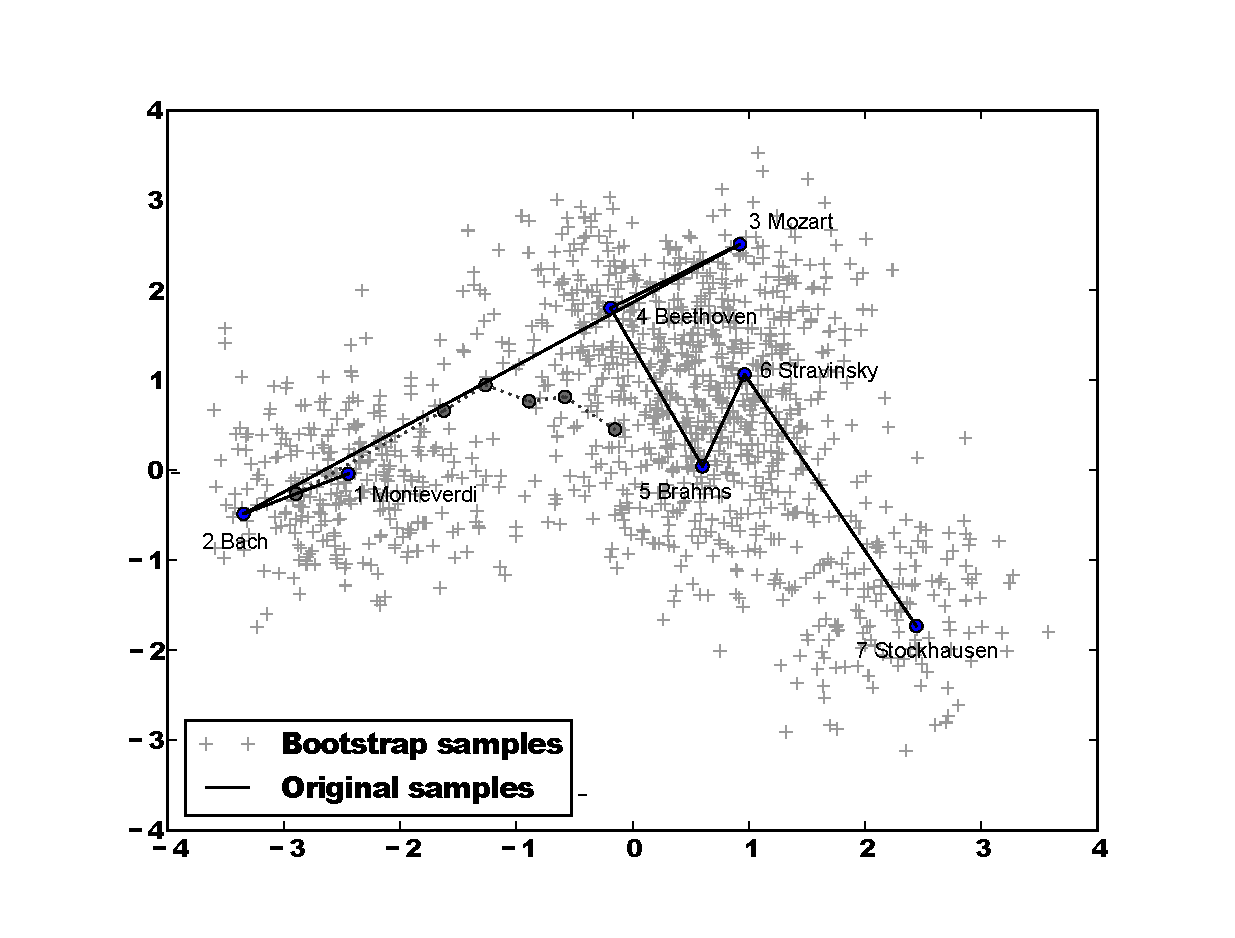
\includegraphics[width=0.45\textwidth]{g1}
  \end{center}
  \caption{\it 2-dimensional projected musical space.}
  \label{fig:pcamus}
\end{figure}

\begin{figure}
        \begin{center}
                \includegraphics[width=0.45\textwidth]{pca_filosofos_novo}
        \end{center}
        \caption{\it 2-dimensional projected philosophical space.}
        \label{fig:pcaphi}
\end{figure}

Starting by analyzing the musical space, Bach is found far from the rest of
composers, which suggests his key role
acknowledged by other great composers like Beethoven and
Webern~\cite{Webern}: ``In fact Bach composed everything, concerned
himself with everything that gives food for thought!''. 
The greatest subsequent change takes place from Bach to Mozart,
reflecting a substantial difference in style.
We can identify a strong relationship between
Beethoven and Brahms, supporting the belief by the \textit{virtuosi} Hans von B\"{u}low~\cite{Bulow} when he
stated the $1^{st}$ Symphony of Brahms as, in reality, being the \textit{$10^{th}$ Symphony of
Beethoven}, clamming Brahms as the true successor of
Beethoven. Stravinsky is near to Beethoven and Brahms,
presumably due to his heterogeneity~\cite{BennettHistory,
  Lovelock}. Beethoven is also near to Mozart who deeply influenced
Beethoven, mainly in his early works.
For Webern, Beethoven was the unique classicist who really came close
to the coherence found in the pieces of the Burgundian School: ``Not even
in Haydn and Mozart do we see these two forms as clearly as in
Beethoven. The period and the eight-bar sentence are at their purest
in Beethoven; in his predecessors we find only traces of them''~\cite{Webern}. It
could explain the proximity of Beethoven to the Renaissance  Monteverdi.
Stockhausen is a deviating point when compared with the others and it
could present even more detachment if we had considered
vanguard characteristics --- e.g.\ timbre exploration by using
electronic devices~\cite{Lovelock} --- not
shared by his precursors.
To complement the analysis of musicians, Table \ref{tab:tableOImus} gives the
opposition and skewness indices for each of the six musical moves,
showing the movements are driven by rather small opposition and strong
skewness. In other words, most musical moves seems to seek more innovation
than opposition. Dialectics is also shown in Table
\ref{tab:tableEmus} and will play a key role in the next section.

\begin{table}[ht]
\caption{\label{tab:tableOImus}Opposition and skewness indices for each
of the six musical moves.}
\begin{tabular}{|c||c|c|}
\hline
Musical Move & $W_{i,j}$ & $s_{i,j}$ \\
\hline \hline
 Monteverdi $\to$ Bach             &   1.0     &  0.      \\
 Bach $\to$ Mozart                 &   1.0196  &  1.9042  \\
 Mozart $\to$ Beethoven            &   0.4991  &  2.8665  \\
 Beethoven $\to$ Brahms            &   0.2669  &  1.7495  \\
 Brahms $\to$ Stravinsky           &   0.4582  &  2.6844  \\
 Stravinsky $\to$ Stockhausen      &   0.2516  &  3.1348  \\
\hline
\end{tabular}
\end{table}

\begin{table}[ht]
\caption{\label{tab:tableEmus} Counter-dialectics index for each
of the five subsequent pairs of musical moves considering the 8 components.}
\begin{tabular}{|c||c|}
\hline
Musical Triple & $d_{i \rightarrow k}$ \\
\hline \hline
 Monteverdi $\to$ Bach $\to$ Mozart          & 2.0586 \\
 Bach $\to$ Mozart $\to$ Beethoven           & 1.2020 \\
 Mozart $\to$ Beethoven $\to$ Brahms         & 1.0769 \\
 Beethoven $\to$ Brahms $\to$ Stravinsky     & 0.2518 \\
 Brahms $\to$ Stravinsky $\to$ Stockhausen   & 0.2549 \\
\hline
\end{tabular}
\end{table}

While analyzing philosophy by opposition and skewness indices, shown in Table \ref{tab:tableOIphi}, all the philosophical moves tend to take place according to a well-defined and intense opposition from the average state.  Also
surprisingly, rather small skewness has been found to underlie most
philosophical moves, meaning that most philosophical moves are driven
almost exclusively by opposition to the current philosophical state.
Remarkable results have been obtained also for dialectics shown in Table \ref{tab:tableEphi}.  We identified progressively stronger dialectics trends among subsequent pairs of philosophical moves.

\begin{table}%\footnotesize%\scriptsize%\tiny
\caption{\label{tab:tableOIphi}Opposition and skewness indices for each
of the six philosophical moves.  }

% \begin{ruledtabular}
\begin{tabular}{|c||c|c|}
\hline
Philosophical Move & $W_{i,j}$ & $s_{i,j}$ \\
\hline \hline
Plato $\rightarrow$ Aristotle     & 1.0    & 0 \\
Aristotle $\rightarrow$ Descartes & 0.8740 & 1.1205 \\
Descartes $\rightarrow$ Espinoza  & 0.9137 & 2.3856 \\
Espinoza $\rightarrow$ Kant       & 0.6014 & 1.6842 \\
Kant $\rightarrow$ Nietzsche      & 1.1102 & 2.9716 \\
Nietzsche $\rightarrow$ Deleuze   & 0.3584 & 2.4890 \\
\hline
\end{tabular}
% \end{ruledtabular}
\end{table}

\begin{table}%\footnotesize%\scriptsize%\tiny
\caption{\label{tab:tableEphi} Counter-dialectics index for each
of the five subsequent pairs of philosophical moves.  }

\begin{tabular}{|c||c|}
\hline
Philosophical Triple & $d_{i \rightarrow k}$ \\
\hline \hline
Plato $\rightarrow$ Aristotle $\rightarrow$ Descartes    & 3.0198 \\
Aristotle $\rightarrow$ Descartes $\rightarrow$ Espinoza & 1.8916 \\
Descartes $\rightarrow$ Espinoza $\rightarrow$ Kant      & 1.1536 \\
Espinoza $\rightarrow$ Kant $\rightarrow$ Nietzsche      & 1.1530 \\
Kant $\rightarrow$ Nietzsche $\rightarrow$ Deleuze       & 0.2705 \\
\hline
\end{tabular}
% \end{ruledtabular}
\end{table}

In order to complement our analysis of the relationship between the composers and philosophers pairs and triples, we performed Wards hierarchical
clustering~\cite{Ward} to complement the analysis. This algorithm clusters the original scores taking into
account their distance. The generated dendrogram in
Figure \ref{fig:dendrogrammus} shows the composers
considering their similarity, the same to philosophers presented on Figure \ref{fig:dendrogramphi}. The representation supports the
observations discussed previously. It is interesting to note the cluster
formed by Beethoven and Brahms, reflecting their heritage. Stravinsky
and Stockhausen forms another cluster and Mozart remains in isolation,
as like Bach and Monteverdi. Both relations were also present in the
planar space shown in Figure \ref{fig:pcamus}.

\begin{figure}[ht]
        \begin{center}
          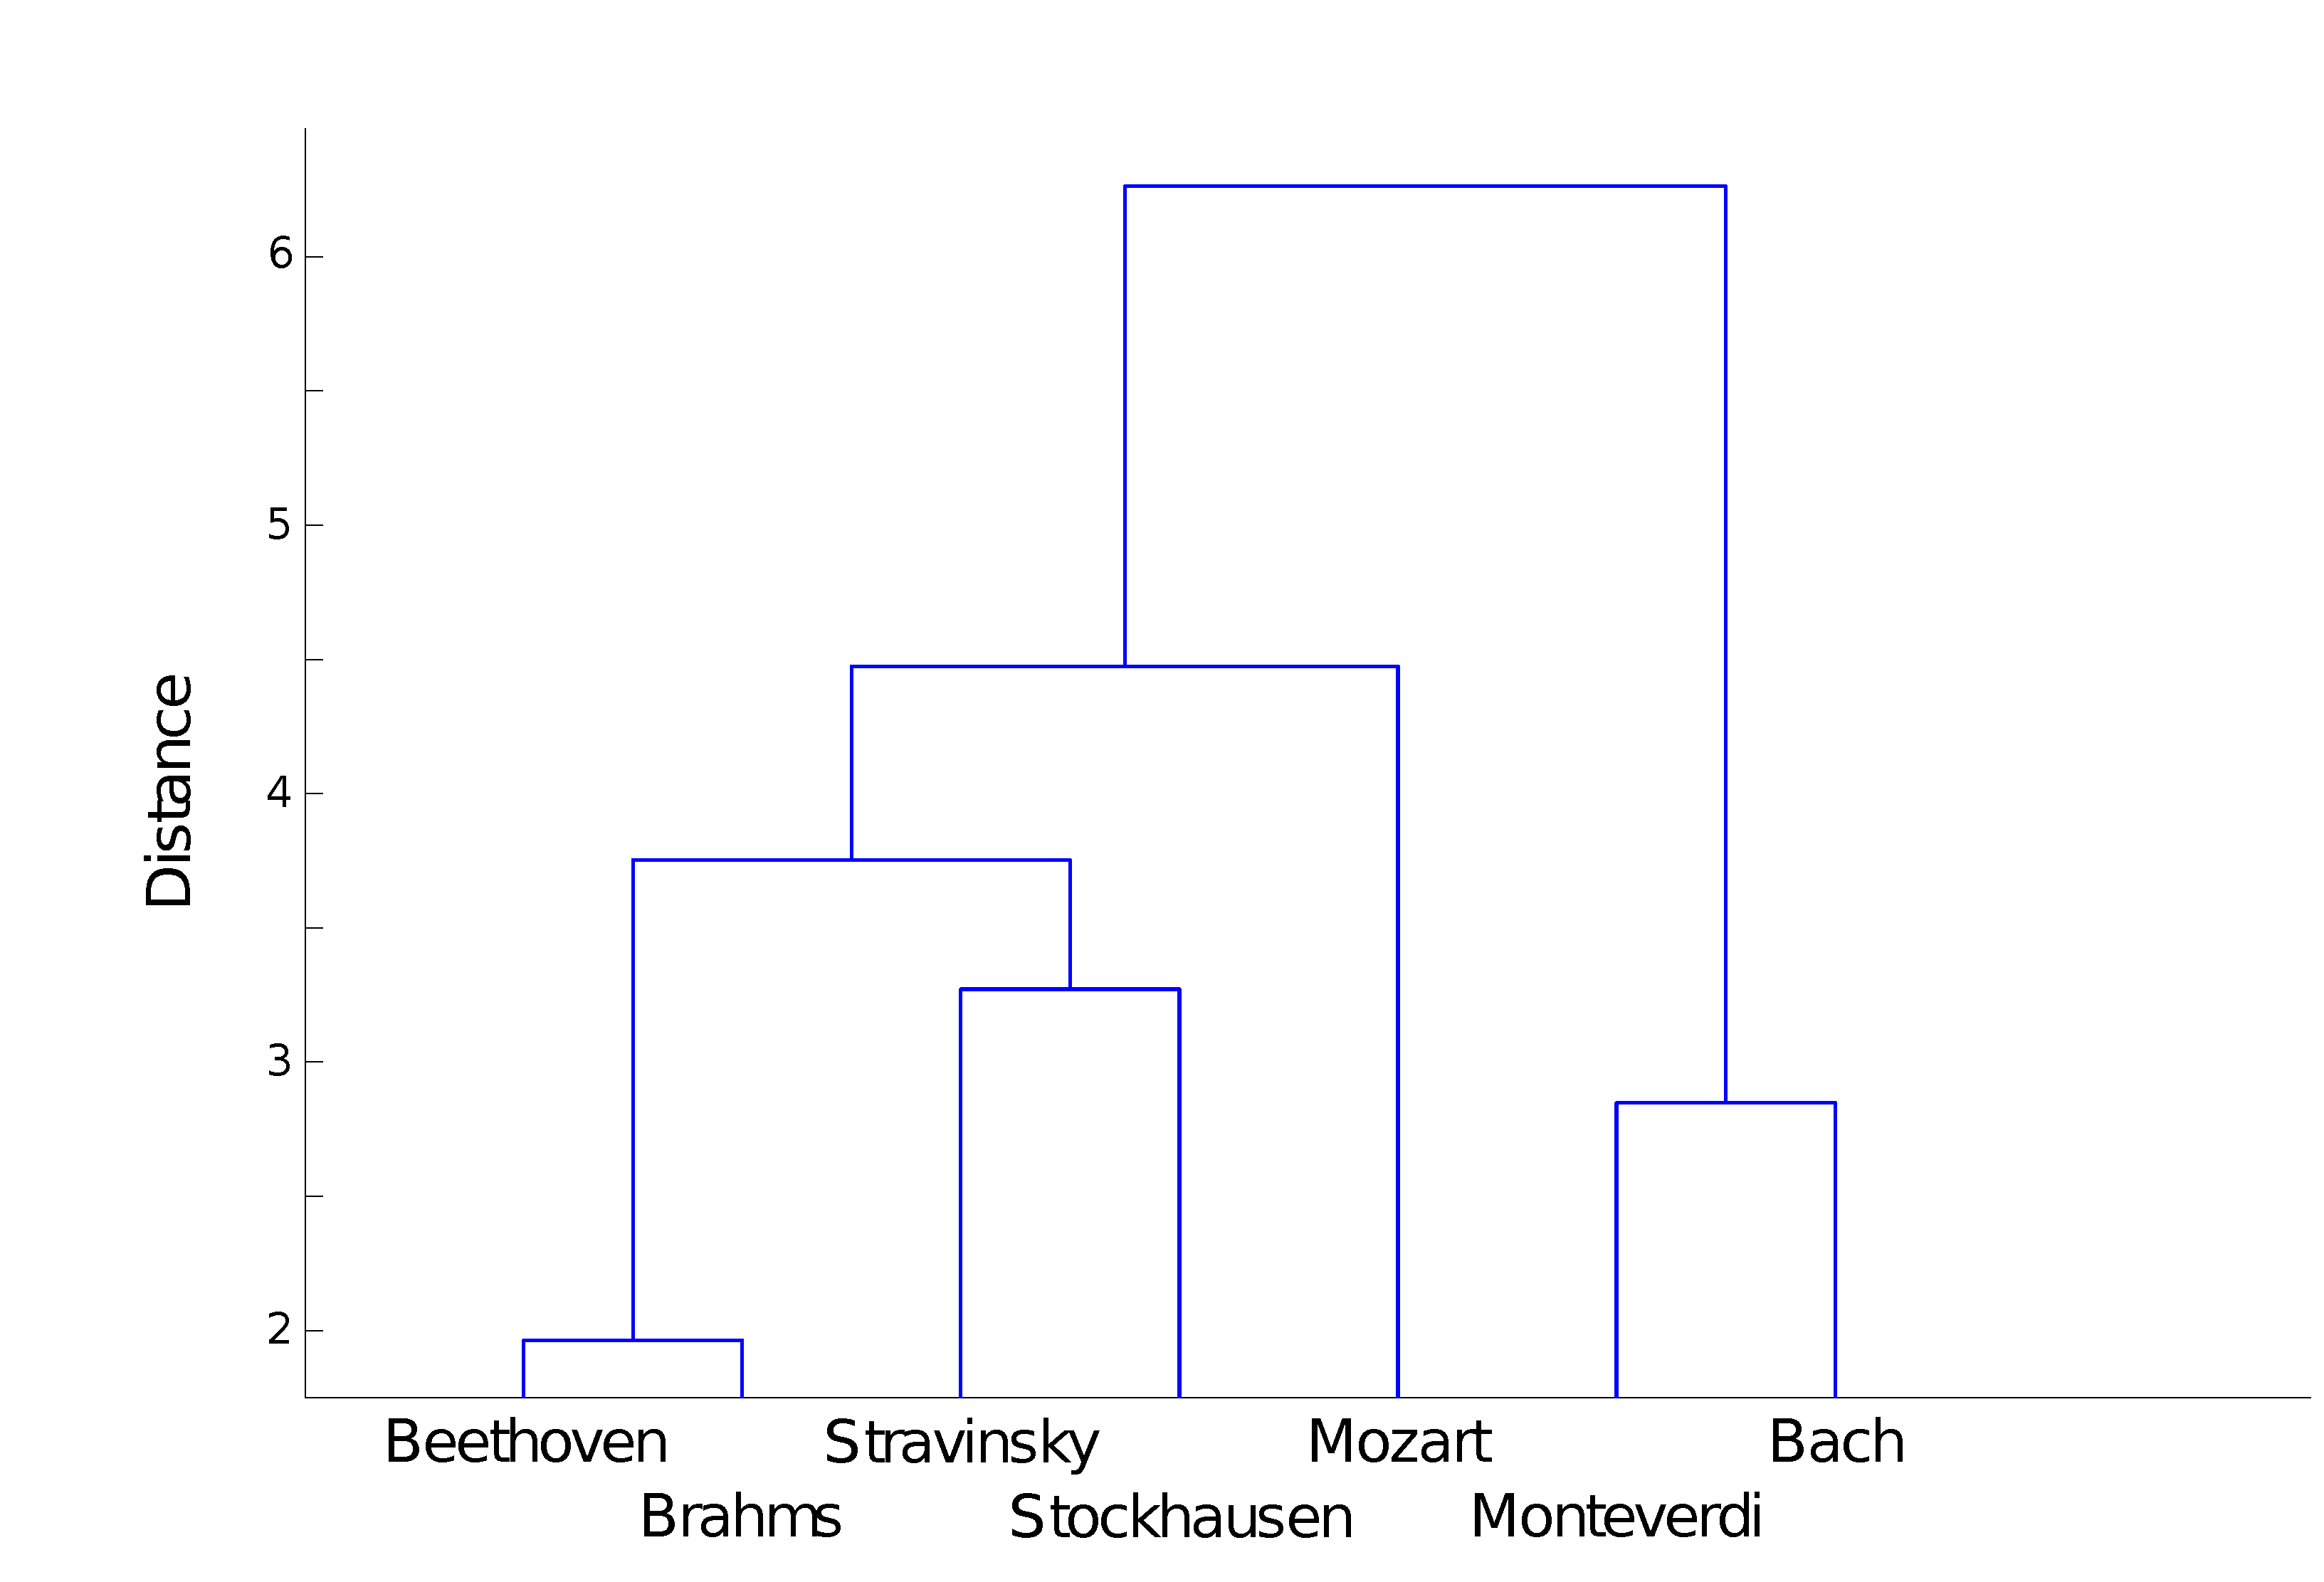
\includegraphics[width=0.45\textwidth]{Clust_Compositores.eps}
        \end{center}
        \caption{\it Wards hierarchical clustering of the seven composers.}
        \label{fig:dendrogrammus}
\end{figure}

\begin{figure}
        \begin{center}
                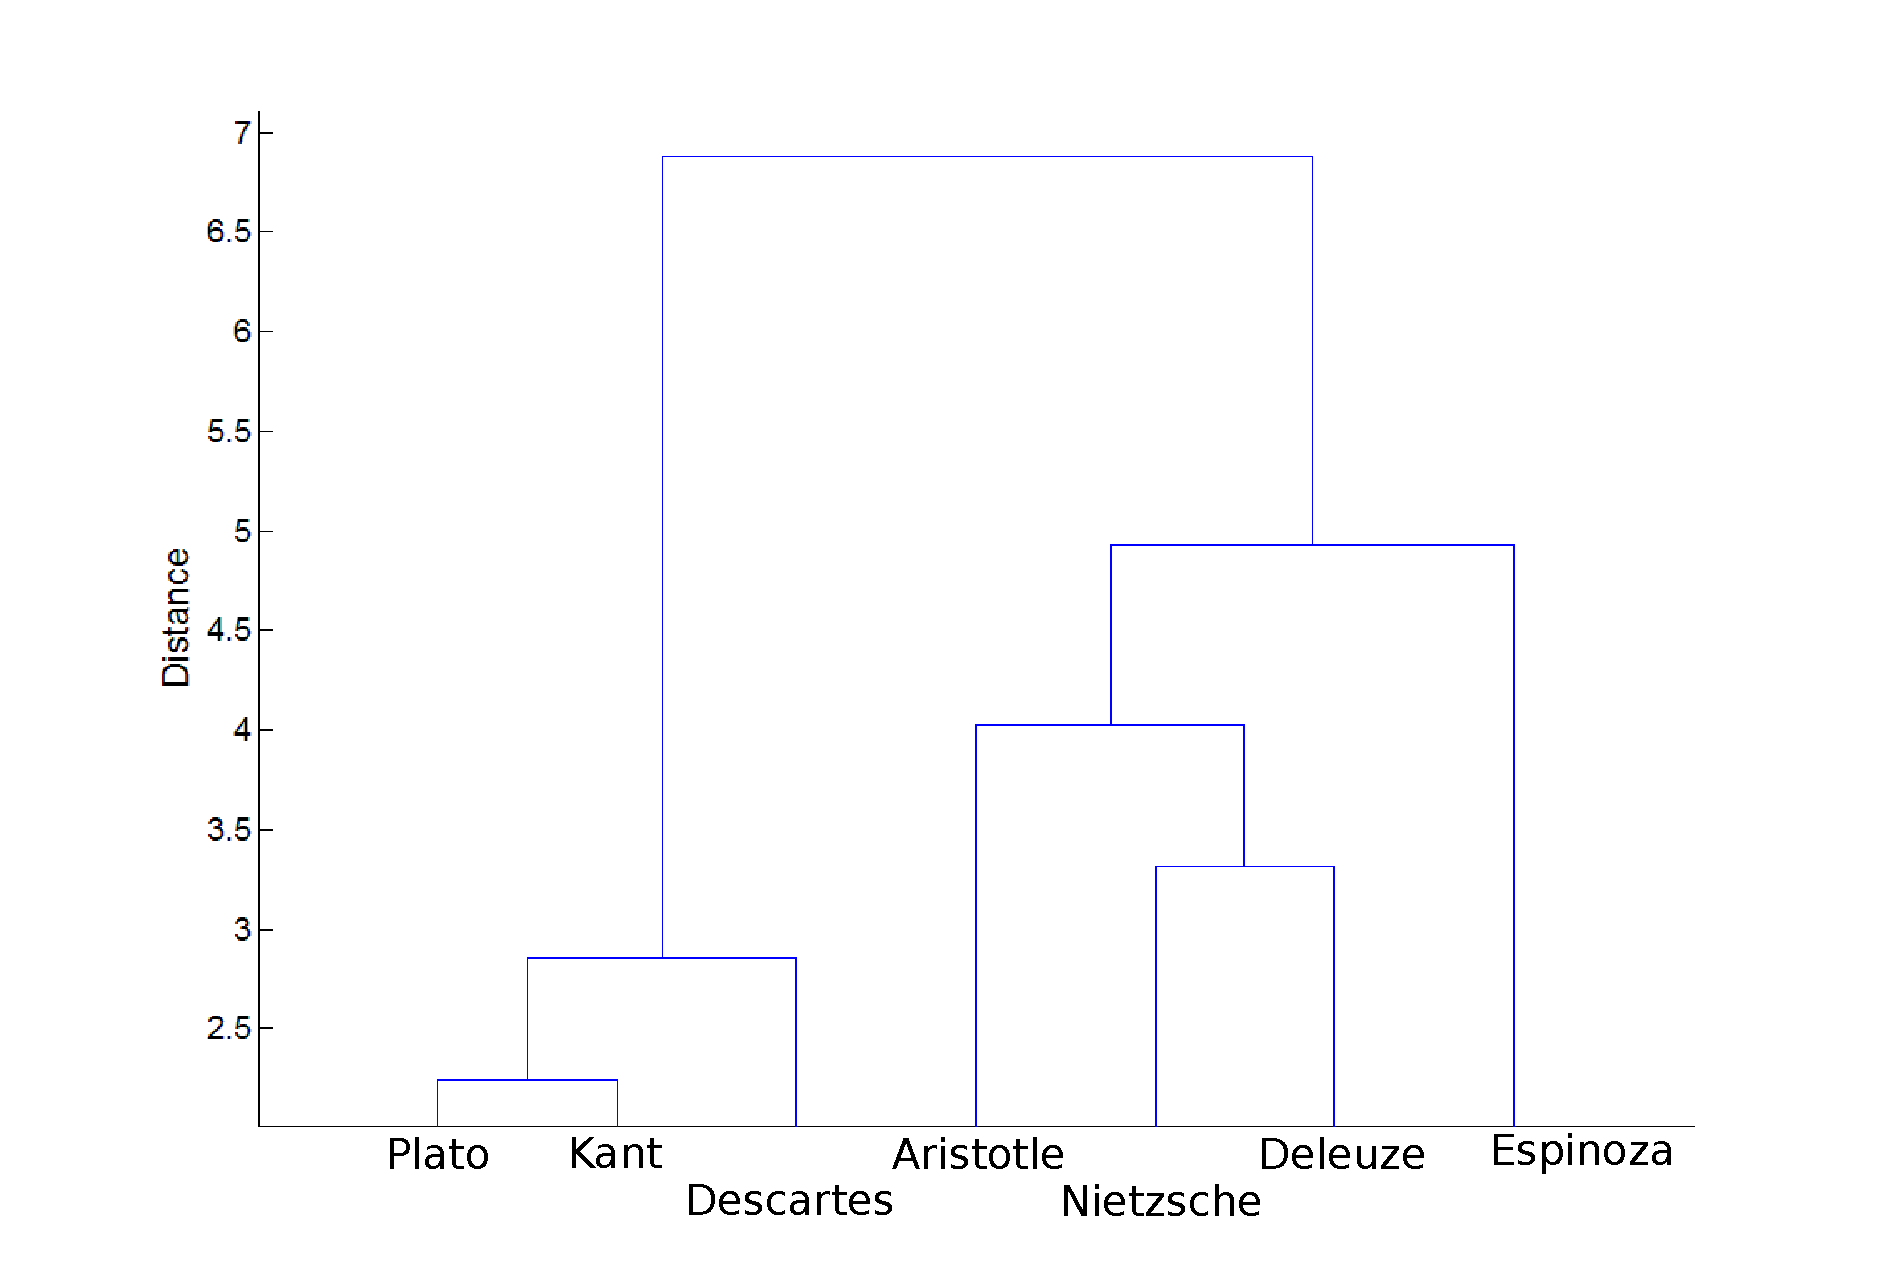
\includegraphics[width=0.5\textwidth]{Dendrogram_.eps}
        \end{center}
        \caption{\it Wards  hierarchical clustering of the seven
                    philosophers considering all the eight features.}
        \label{fig:dendrogramphi}
\end{figure}

\section{Comparisons with Philosophers Analysis}

The results of composers analysis are surprising when compared with philosophers. It is important to note that we preserved the
number of characteristics and performed the same bootstrap method to
generate a larger set of samples, making possible this
comparison. The variances after PCA (Table \ref{tab:tableCphi}) concentrates in the four first new axis, similar to the variances for composers shown at Table \ref{tab:tableCphi}. If we compare the discussed musical space (Figure \ref{fig:pcamus})
with the philosophical one in Figure \ref{fig:pcaphi} we
identify opposite movements along all the philosophy history in contrast
to music. This reveals a notorious characteristic of the way
philosophers seem to have evolved their ideas, driven by opposition ($W_{i,j}$), as shown in Table \ref{tab:tableOIphi}, while
composers tend to be more influenced by their predecessors as far as their dialectics measures are
concerned ($1/d_{i \rightarrow k}$).
In general, the musical movements had minor opposition and,
remembering the beginning of this work, it reflects the
master-apprentice
tradition present in music: the composers tend to build their own
works confirming their precursors legacy, resulting in a greater
dialectics than the philosophers related measures.
This reveals a crucial difference
considering the \textit{memory treatment} along the development of
philosophy and music: using the same techniques,
we could verify that a philosopher was influenced by the
opposition of ideas from his direct predecessor, while here composers were commonly
influenced by their both predecessors. Therefore, we can argue that philosophy
presents a \textit{memory-1} state, while music presents
\textit{memory-2}, considering \textit{memory-N} being as number $N$
of past generations whose influence on a philosopher or
composer is being considered. Considering the linearity of musical movements we can
identify the abscissa as a ``time axis'' representing the development
of music along the history, with some composers
like Beethoven returning to Monteverdi and others advancing to the
modern age like Stravinsky and Stockhausen.

The opposition and skewness indices for philosophers listed in Table
\ref{tab:tableOIphi} endorses the minor role of opposition in
composers at the period considered. We can observe strong opposition
in philosophical moves contrasted to small opposition in
musical movements. Also, the dialectics presents a
phase difference suggesting knownledge and aesthetics 
transfer latency between each of these human fields.

When comparing dialectics, other curious facts arise: the dialectics
indices for musicians in Table \ref{tab:tableEmus} are considerably stronger moves than for
philosophers in Table \ref{tab:tableEphi}. Both indices are also shown in Figure
\ref{fig:comparingdialectics} where we can see a constant decrease
of counter-dialectics. This makes it possible to argue
that dialectics is stronger in music where a
constantly return to the origins are clearly visible. This reveals the nature of the
musical development, based on the search for a unity. Using the words
of Webern, the search for the ``comprehensibility'' but always
influenced by their old masters.

\begin{figure}[ht]
        \begin{center}
                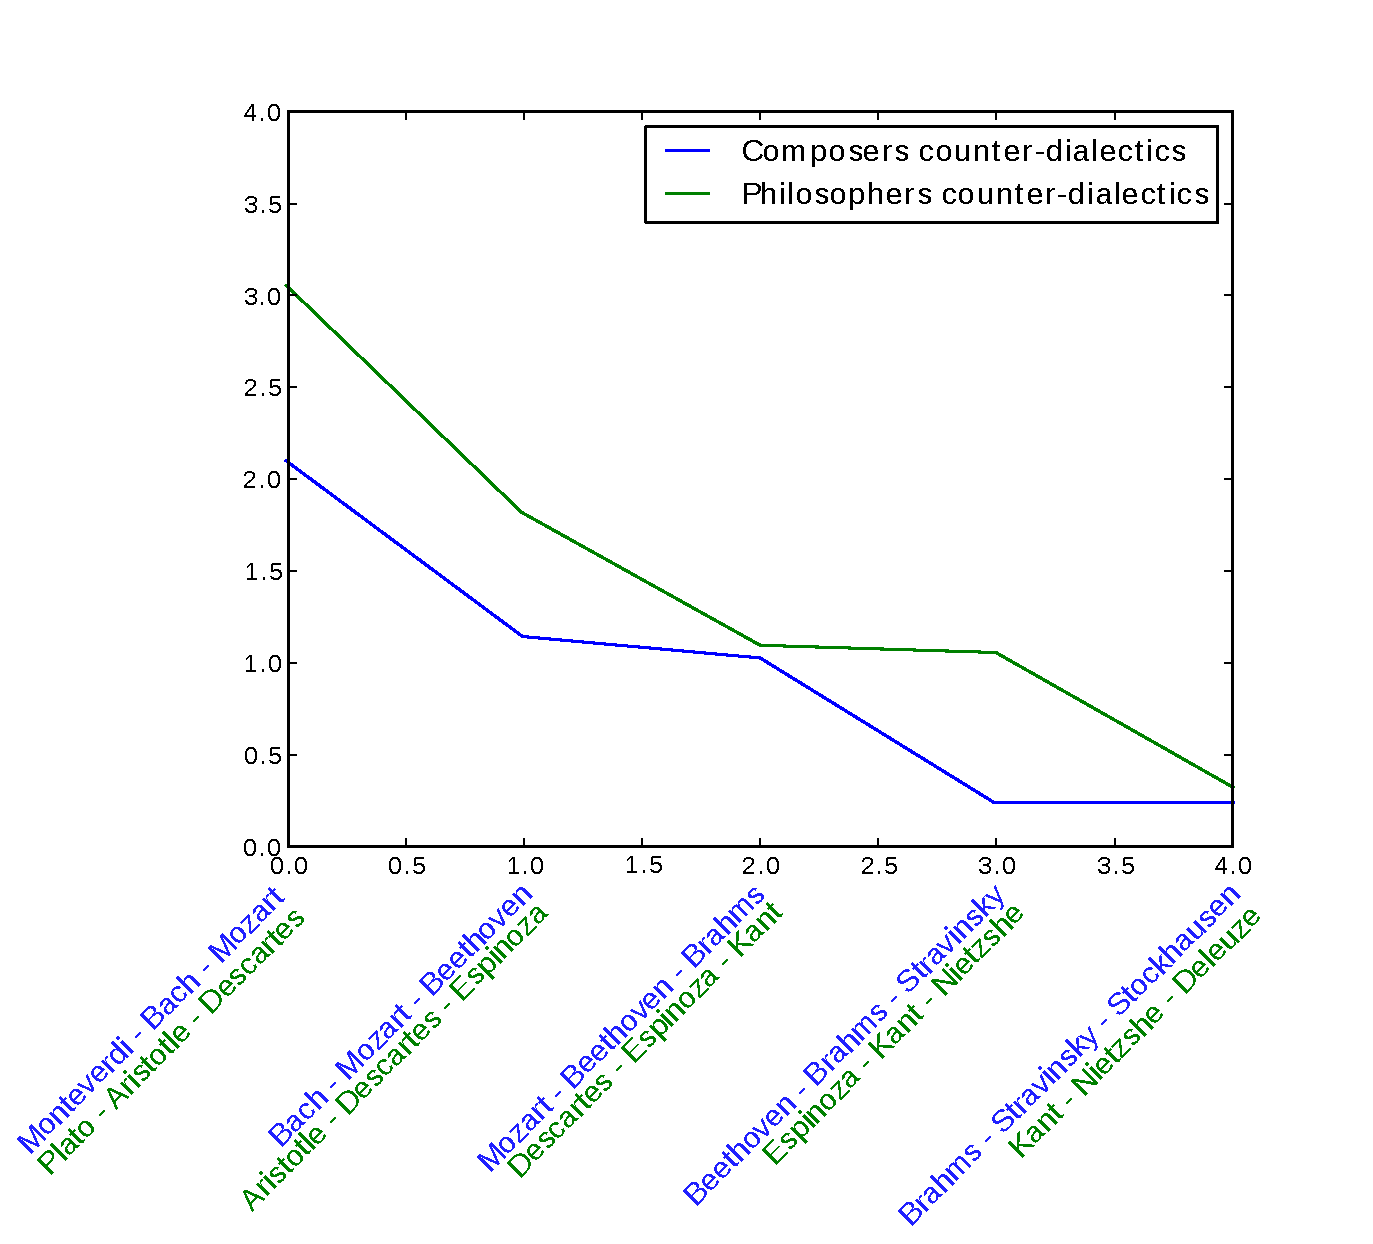
\includegraphics[width=0.45\textwidth]{compara_dialeticas2}
        \end{center}
        \caption{\it Comparison between composers and philosophers
          counter-dialectics indices}
        \label{fig:comparingdialectics}
\end{figure}

\section{Concluding Remarks}

Motivated by the understanding of how humanities evolves, we proposed a quantitative method and applied that in two case studies: music and philosophy. Statistical
methods is nowadays commonly used for the study of music features and
composers productivity, but analysis of
composers characteristics modification along the music history has been less
explored. Automatic information retrieval techniques while common in music analysis are fewer on philosophy considering the nature of final products of both fields. The method proposed here differs on the
aspect of how the characteristics concerning composers are treated:
scores are assigned to each feature common in musical
works. 

It should be acknowledged that the scores and choice of main
musical or philosophical characteristics adopted in the current work are largely
arbitrary and could be substantially improved.  However, the
perturbation analysis performed in this work suggests that the effect
of non-systematic errors in assigning the scores does not seem to be
critical and has little overall impact on the conclusions we have
derived.  In addition, whatever the effects of the scores and choice
of main features, it should be emphasized that the proposed
methodology can be readily applied to expanded and enhanced sets of
scores or musical and philosophical characteristics.  As a matter of fact, this is
perhaps the main contribution of this work, i.e.\ the proposal of a
sound, formal quantitative methodology which can lead to
comprehensive, objective insights about how humanities fields has evolved
since its earliest origins.  It is also worth observing that this
methodology is not restricted to individual composers or philosophers, and it can
be adapted to the investigation of musical and philosophical schools, individual
pieces (e.g.\ music suites or books), or even of the works of the same composers or philosophers
along distinct periods of time.  It is also possible to apply this
methodology to other areas such as poetry, cinema and science.
These scores reveal not the
exact profile of composers, but a tendency of how their
techniques are usually present. Information retrieval techniques could be considered to make the study stronger, but the current method gives an \emph{initial guess} based on reviewers opinion. 

To make the simulation more
realistic, we considered not just the small number of 7 original samples, but
derived other 1000 new ``artificial samples'' through a bootstrap
method. A larger data set made possible the statistical analysis,
considering not just the original scored composers or philosophers, but other samples
that respect the historical presence of the formers. This other thousand
entities were modeled by a
probabilistic distribution, and avoided a biasing caused by
the use of only 7 samples.
In order to investigate the
relationship between this scorings we applied Pearson correlation
analysis. The results demonstrated a strong correlation between some
characteristics, which allows us to group this values, creating a
reduced number of features that summarizes the most important
characteristics. PCA was also applied to these components, reducing
the complex space to a planar graph where some of the most interesting
properties can be visualized. 
Historical landmarks in both music and philosophy are
well-defined in the planar space, like the isolation of Bach, Mozart
and Stockhausen, the
proximity between Beethoven and Brahms and the distance from Bach and Mozart, the heterogeneity of
Stravinsky and the vanguard of contemporary composers
like Stockhausen. Even not so visible relations, like the trend to return to the maximum domain of polyphony -- present on Renaissance -- by Beethoven
could also be clearly observable, demonstrating the chronological nature of the
space. 
The dichotomy between
master-apprentice tradition on music and the quest for innovation that
opened this discussion could be visualized quantitatively. Each
composer demonstrated his own style, differing considerably from his
predecessor -- clearly shown when analyzing pairs of subsequent composers like
Bach and Mozart, Mozart and Beethoven or Stravinsky and
Stockhausen. Otherwise, the inheritance of predecessors styles is also
present when analyzing the direct relations between Mozart and
Beethoven or Beethoven and
Brahms, or indirect ones between Bach and Beethoven
or Beethoven and Monteverdi. The entire scenario presented
a ``continual pattern'' between
composers -- motivated by the influence of theirs predecessors -- but also showed a force
repelling both of them: the innovation, or in the words of William
Lovelock~\cite{Lovelock}, the ``experimentation'' that makes progress possible.
Along the analysis we noticed interesting differences when comparing
composers with philosophers. While on philosophy the
innovation is notably marked by opposition of each philosophers ideas,
it is less present for music composers. The lack of strong
opposition movements and proeminent presence of dialectics in musical space indicates the music innovation is driven by
a constant heritage of each composer from his predecessors. We
represented this characteristic referring to a \textit{memory state}
where philosophers shows \textit{memory-1} -- each philosopher was
influenced by opposite ideas of its direct predecessor -- while
composers shows \textit{memory-2} -- inheriting the style of their
both direct predecessors.
The
analysis of both dialectics values also shown surprising
results: on philosophy the dialectics indices are arranged on a
increasing series -- showing a strong influence of
dialectics to philosophy development -- the dialectics indices on
music exhibits the same pattern, but with an offset. This behavior presumably indicates a
constant quest for coherence by the composers, a fact notably observed by
the studies of Anton Webern~\cite{Webern} should have somewhat the same
kernel and a lattency between the effects.
Another result is that the quantitative methodology initially applied to the analysis of philosophy~\cite{Fabbri}
proved to be extensible to other fields of knowledge -- in this case music --
reflecting with considerable efficiency details concerning the specific field. 
Computational analysis of music scores could be
applied to automate the quantification of composers characteristics, like
identification of melodic and harmonic patterns or the presence or not of
polyrhythms, motivic and harmonic stability~\cite{Correa}. More composers could be
inserted in the set for the analysis of a wider time-line, possibly
including more representatives of each music period.
% While taking the first
% steps on the direction of a quantitative approach to analising arts and philosophy
% our aim is to quantify creativity evolution.
We want to end this work going back to Webern,
who early envisioned these relations: ``It is clear that where relatedness and unity are omnipresent,
comprehensibility is also guaranteed. And all the rest is
dilettantism, nothing else, for all time, and always has been. That's
so not only in music but everywhere.''
\begin{acknowledgments}
Luciano da F. Costa thanks CNPq (308231/03-1) and FAPESP (05/00587-5)
for sponsorship. Gonzalo Travieso thanks CNPq (308118/2010-3) for sponsorship. 
Vilson Vieira and Renato Fabbri is grateful to CAPES and 
the Postgrad Committee of the IFSC.
\end{acknowledgments}

\appendix

\section{A Brief Explanantion of Principal Component Analysis (PCA)}

In plain words, PCA is a dimensionality reduction procedure performed
through axes rotation.  It operates by concentrating
dispersion/variance along the first new axes, which are denominated
the principal components.

The technique consists in finding the eigenvectors and eigenvalues of
the covariance matrix of the respective random vectors (i.e.\ the
vectors associated with each philosophical state). The eigenvalues
correspond to the variances of the new variables.  When multiplied by
the original feature matrix, the eigenvectors yield the new random
variables which are fully uncorrelated.

For a more extensive explanation of PCA, please refer to~\cite{Costa}
and references therein.

\nocite{*}
\bibliography{phi+mus}
\end{document}
